\documentclass[journal,12pt,twocolumn]{IEEEtran}
%

\usepackage{setspace}
\usepackage{gensymb}
\singlespacing

\usepackage{amsmath}
\usepackage{amsthm}
\usepackage{txfonts}
\usepackage{cite}
\usepackage{enumitem}
\usepackage{mathtools}
\usepackage{hyperref}
\usepackage{listings}
    \usepackage{color}                                            %%
    \usepackage{array}                                            %%
    \usepackage{longtable}                                        %%
    \usepackage{calc}                                             %%
    \usepackage{multirow}                                         %%
    \usepackage{hhline}                                           %%
    \usepackage{ifthen}                                           %%
  %optionally (for landscape tables embedded in another document): %%
    \usepackage{lscape}     
\usepackage{multicol}
\usepackage{chngcntr}
\renewcommand\thesection{\arabic{section}}
\renewcommand\thesubsection{\thesection.\arabic{subsection}}
\renewcommand\thesubsubsection{\thesubsection.\arabic{subsubsection}}

% correct bad hyphenation here
\hyphenation{op-tical net-works semi-conduc-tor}
\def\inputGnumericTable{}                                 %%

\lstset{
%language=C,
frame=single, 
breaklines=true,
columns=fullflexible
}

\begin{document}
%


\newtheorem{theorem}{Theorem}[section]
\newtheorem{problem}{Problem}
\newtheorem{proposition}{Proposition}[section]
\newtheorem{lemma}{Lemma}[section]
\newtheorem{corollary}[theorem]{Corollary}
\newtheorem{example}{Example}[section]
\newtheorem{definition}[problem]{Definition}
\newcommand{\BEQA}{\begin{eqnarray}}
\newcommand{\EEQA}{\end{eqnarray}}
\newcommand{\define}{\stackrel{\triangle}{=}}
\bibliographystyle{IEEEtran}
\providecommand{\mbf}{\mathbf}
\providecommand{\pr}[1]{\ensuremath{\Pr\left(#1\right)}}
\providecommand{\qfunc}[1]{\ensuremath{Q\left(#1\right)}}
\providecommand{\sbrak}[1]{\ensuremath{{}\left[#1\right]}}
\providecommand{\lsbrak}[1]{\ensuremath{{}\left[#1\right.}}
\providecommand{\rsbrak}[1]{\ensuremath{{}\left.#1\right]}}
\providecommand{\brak}[1]{\ensuremath{\left(#1\right)}}
\providecommand{\lbrak}[1]{\ensuremath{\left(#1\right.}}
\providecommand{\rbrak}[1]{\ensuremath{\left.#1\right)}}
\providecommand{\cbrak}[1]{\ensuremath{\left\{#1\right\}}}
\providecommand{\lcbrak}[1]{\ensuremath{\left\{#1\right.}}
\providecommand{\rcbrak}[1]{\ensuremath{\left.#1\right\}}}
\theoremstyle{remark}
\newtheorem{rem}{Remark}
\newcommand{\sgn}{\mathop{\mathrm{sgn}}}
\providecommand{\abs}[1]{\lvert#1\rvert}
\providecommand{\res}[1]{\Res\displaylimits_{#1}} 
\providecommand{\norm}[1]{\lVert#1\rVert}
\providecommand{\mtx}[1]{\mathbf{#1}}
% \providecommand{\mean}[1]{E\left[ #1 \right]}
\providecommand{\fourier}{\overset{\mathcal{F}}{ \rightleftharpoons}}
\providecommand{\system}{\overset{\mathcal{H}}{ \longleftrightarrow}}
\newcommand{\solution}{\noindent \textbf{Solution: }}
\newcommand{\cosec}{\,\text{cosec}\,}
\providecommand{\dec}[2]{\ensuremath{\overset{#1}{\underset{#2}{\gtrless}}}}
\newcommand{\myvec}[1]{\ensuremath{\begin{pmatrix}#1\end{pmatrix}}}
\newcommand{\cmyvec}[1]{\ensuremath{\begin{pmatrix*}[c]#1\end{pmatrix*}}}
\newcommand{\mydet}[1]{\ensuremath{\begin{vmatrix}#1\end{vmatrix}}}
\newcommand{\proj}[2]{\textbf{proj}_{\vec{#1}}\vec{#2}}
\newcommand{\RNum}[1]{\uppercase\expandafter{\romannumeral #1\relax}}
\let\StandardTheFigure\thefigure
\let\vec\mathbf


\title{
Assignment 2
}
\author{ Rishabh Bhardwaj \\SM21MTECH12007}
\maketitle
\newpage
\bigskip
\bibliographystyle{IEEEtran}
\section{ chapter \RNum{3}  miscellaneous examples \RNum{6} Q6 }
\noindent
\textbf{\textsl{Find the area of parallelogram formed by the lines}}
$$$$
\textbf{\textsl{i. 12x - 5y = 7a,\\ ii. 5x - 12y = -7a,\\ iii. 5x - 12y = -126a,\\ iv. 12x - 5y = 126a}}
\noindent
\section*{\textbf{Solution}}
\noindent
% First, we need to find the intersection point of given three lines, \\
\\
Let's find the intersection of line (i) and (ii),\\
\\
In matrix form, we have
\begin{align*}
\vec{A}\vec{M} &=\vec{B} \\
\vec{M} &= \vec{A}^{-1}\vec{B} \\
\vec{M}
& =
\begin{bmatrix}
12 & -5 \\
5 & -12 
\end{bmatrix}^{-1}
\begin{bmatrix}
7a\\ -7a
\end{bmatrix}  \\[6pt]
\vec{M}
& =
\frac{-1}{119}
\begin{bmatrix}
-12 & 15 \\
-5 & 12 
\end{bmatrix}
\begin{bmatrix}
7a \\ -7a
\end{bmatrix} \\[6pt]
\vec{M}
&=
\begin{bmatrix}
a \\ a
\end{bmatrix}
\end{align*}
Similarly solving for lines (i) and (iii), we get
\begin{align*}
\vec{A}\vec{N} &=\vec{C} \\
\vec{N} &= \vec{A}^{-1}\vec{C} \\
\vec{N}
& =
\begin{bmatrix}
12 & -5 \\
5 & -12 
\end{bmatrix}^{-1}
\begin{bmatrix}
7a \\ -126a
\end{bmatrix}  \\[6pt]
\vec{N}
& =
\frac{-1}{119}
\begin{bmatrix}
-12 & 5 \\
-5 & 12 
\end{bmatrix}
\begin{bmatrix}
7a \\ -126a
\end{bmatrix} \\[6pt]
\vec{N}
&=
\begin{bmatrix}
6a \\ 13a
\end{bmatrix}
\end{align*}
Similarly solving for lines (ii) and (iv), we get
\begin{align*}
\vec{E}\vec{P} &=\vec{D} \\
\vec{P} &= \vec{E}^{-1}\vec{D} \\
\vec{P}
& =
\begin{bmatrix}
5 & -12 \\
12 & -5 
\end{bmatrix}^{-1}
\begin{bmatrix}
-7a \\ 126a
\end{bmatrix}  \\[6pt]
\vec{P}
& =
\frac{1}{119}
\begin{bmatrix}
-5 & 12 \\
-12 & 5 
\end{bmatrix}
\begin{bmatrix}
-7a \\ 126a
\end{bmatrix} \\[6pt]
\vec{P}
&=
\begin{bmatrix}
13a \\ 6a
\end{bmatrix}
\end{align*}\\ \\
The area of the $\parallel$gm is given by the norm $$\norm{\vec{NM}\times\vec{PM}} $$
Since, \\
\vec{NM} = \myvec{5a\\12a}\\
\vec{PM} = \myvec{12a\\5a}\\
Therefore, \\
\begin{align*}
\vec{NM}\times\vec{PM}&=\myvec{25a^2 - 144a^2}\\
&={-119a^2}
\end{align*}

Eventually we get \textbf{Area} = $119a^2$ units
\begin{figure}[!ht]
	\centering
	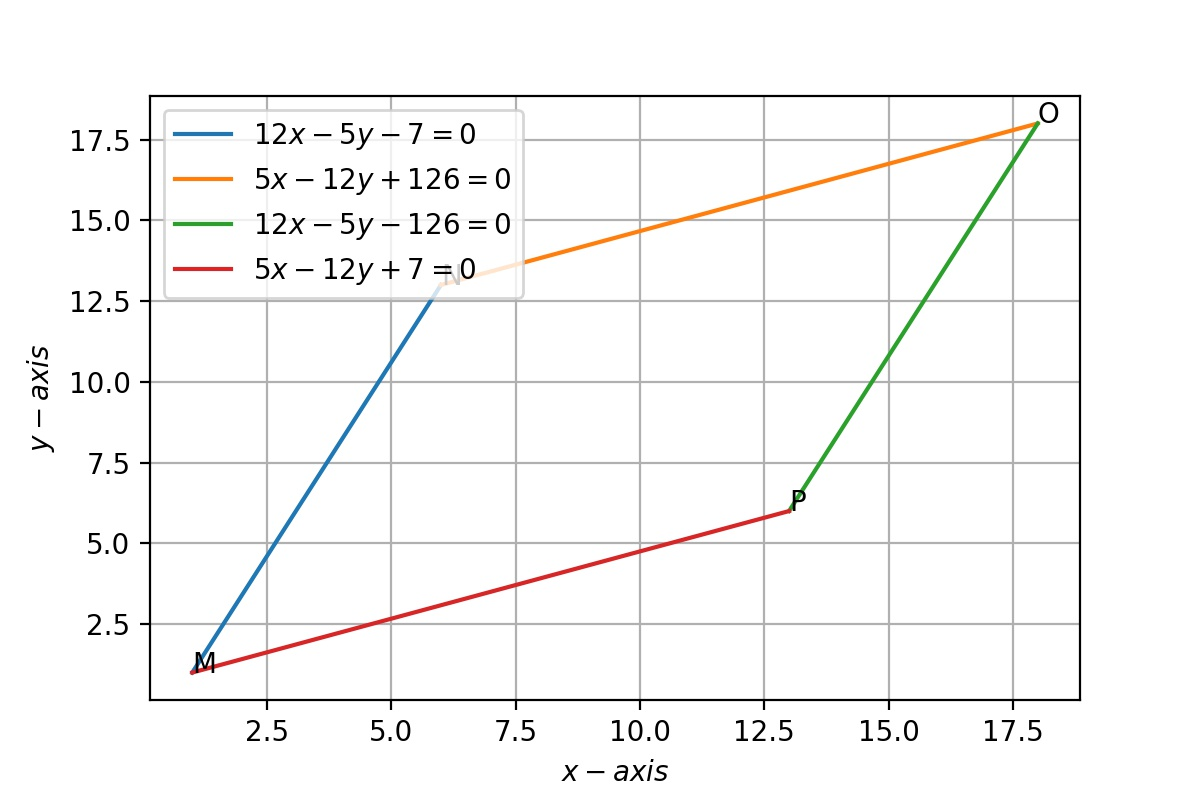
\includegraphics[width=\columnwidth]{parallelogram.jpg}
	\caption{The parallelogram formed by the given lines}
	\label{fig:parallelogram}
\end{figure}


\end{document}
